\chapter{METODOLOGÍA DE LA INVESTIGACIÓN}

\section{Diseño de la investigación}

En esta sección se describirá el diseño de la investigación, el cual incluirá el alcance, enfoque y tipo de estudio que se realizará. Asimismo, se detallarán la población y muestra que serán consideradas en este trabajo.

\subsection{Alcance de la investigación}
El presente estudio tendrá un alcance explicativo, ya que se analizará cómo la aplicación de técnicas avanzadas de procesamiento de imágenes y algoritmos de clustering contribuirá a la automatización en la generación de clips informativos a partir de videos de noticias. Se buscará identificar patrones visuales y explicar cómo estos representan eventos clave en las noticias. El uso de técnicas como HOG para la extracción de características y K-means para el agrupamiento de frames permitirá optimizar la selección de contenido relevante en un entorno con sobrecarga informativa.

\subsection{Tipo de investigación}
Este estudio será de tipo no experimental, ya que no se manipularán deliberadamente las variables independientes ni se ejercerá control sobre los factores involucrados en el fenómeno estudiado. Los datos se observarán y analizarán en su contexto natural, específicamente los videos de noticias obtenidos de plataformas como YouTube. El análisis se centrará en la aplicación de técnicas de procesamiento de imágenes y algoritmos de clustering para identificar patrones y agrupar frames representativos, sin intervenir en las condiciones de producción de los videos ni en los eventos que presentan.

\subsection{Enfoque de investigación}
El enfoque de esta investigación será cuantitativo, dado que se basará en la recolección y análisis de datos numéricos derivados de los videos de noticias procesados. A través de la implementación de técnicas de procesamiento de imágenes y algoritmos de clustering, se buscará medir, agrupar y analizar objetivamente los frames más representativos para la generación automática de clips informativos.
\section{Población y muestra}

\begin{table}[H]
	\centering
	\caption{Descripción del estudio}
	\begin{tabular}{p{5cm}p{10cm}}
		\hline
		\textbf{Categoría} & \textbf{Descripción} \\ \hline
		\textbf{Población} & Videos de noticias disponibles en plataformas como YouTube que cubrirán eventos de actualidad a nivel nacional e internacional. \\ \hline
		\textbf{Muestra} & 
		\begin{itemize}
			\item 40 vídeos de noticias en formato MP4 que serán extraídos automáticamente de YouTube utilizando la herramienta Youtube-Dlp.
		\end{itemize}
		\\ \hline
		\textbf{Unidad de análisis} & Un vídeo de noticias completo que contendrá información sobre eventos relevantes de un día específico. \\ \hline
	\end{tabular}
	\label{tabla:poblacion_muestra}
\end{table}

\section{Operacionalización de variables}

\begin{table}[H]
	\centering
	\caption{\textit{Operacionalización de Variables}}
	\begin{adjustbox}{max width=\textwidth}
	\begin{tabular}{p{4cm}p{4cm}p{4cm}p{4cm}}
		\hline
		\textbf{Variable} & \textbf{Dimensión} & \textbf{Indicador} & \textbf{Cálculo} \\ \hline
		\textbf{Independiente: Algoritmo de Clustering} 
		& Datos de entrada & Volumen de datos & Cantidad de videos MP4 \\ \cline{2-4}
		
		\textbf{Dependiente: Creación automática de clips informativos} 
		& Indicadores de desempeño & Inertia & Fórmulas específicas para cada métrica \\ \hline
	\end{tabular}
	\end{adjustbox}
	\label{tabla:operacionalizacion_variables}
\end{table}
\section{Técnicas de recolección}

En esta investigación se emplearán técnicas de recopilación de datos automatizadas que permitirán la obtención eficiente y estructurada de videos de noticias. La herramienta principal que se utilizará será Youtube-DLP, un software de código abierto que facilitará la descarga automatizada de videos en formato MP4 desde plataformas como YouTube. Esta técnica asegurará la recopilación de grandes volúmenes de datos de manera precisa, permitiendo definir criterios específicos como la relevancia del contenido, la fecha de publicación y la duración de los videos, con el objetivo de garantizar que el material recopilado sea pertinente para el análisis de eventos clave. Asimismo, los videos recopilados se almacenarán y organizarán de manera estructurada, incluyendo metadatos como el título y la fuente de los videos, lo que facilitará tanto el acceso como el procesamiento posterior para el análisis automatizado.

\section{Técnicas para el procesamiento y análisis de la información}

\subsection{Metodología de la implementación de la solución}

\begin{figure}[H]
	\centering
	\includegraphics[width=0.9\textwidth]{3/figures/Metodología.png}
	\caption{Metodología del estudio.}
\end{figure}

\subsubsection{Recolección de datos}
La recolección de datos será un componente esencial para el desarrollo de esta investigación. En este proyecto, se recopilarán un total de 36 videos en formato MP4, descargados automáticamente. Estos videos serán extraídos de noticieros en la plataforma YouTube, utilizando la herramienta Youtube-DLP. Los datos recopilados se almacenarán en una carpeta con un límite de tamaño total de 6 GB.

\subsubsection{Preprocesamiento de datos}
El preprocesamiento de datos será crucial para preparar los videos y sus frames recopilados antes de aplicar los modelos de análisis y clustering. Las tareas de preprocesamiento incluirán:

\begin{itemize}
    \item \textbf{Extracción de frames}: Se extraerán frames de los videos con el fin de capturar representaciones visuales relevantes de los eventos y elementos clave presentes en las noticias. Los intervalos de captura se establecerán en función de los frames por segundo.
    \item \textbf{Reducción de frames}: Los frames extraídos serán evaluados para eliminar aquellos que sean irrelevantes o redundantes, como transiciones o escenas sin valor informativo, garantizando que el análisis se enfoque en el contenido más significativo.
    \item \textbf{Normalización}: Los frames serán normalizados en términos de resolución y formato, asegurando que los datos visuales sigan un estándar homogéneo, lo que permitirá que los algoritmos de procesamiento funcionen de manera más eficiente.
    \item \textbf{Etiquetado de frames procesados}: Los frames procesados serán almacenados y etiquetados para facilitar su organización y posterior análisis durante la fase de generación de clips informativos.
\end{itemize}

\subsubsection{Extracción de Características}
La extracción de características será esencial para capturar la información visual relevante de los frames. Se utilizarán dos técnicas complementarias: Histogram of Oriented Gradients (HOG) y Redes Neuronales Convolucionales (CNN), que se integrarán mediante un proceso de stacking para obtener un único vector de características representativo de cada frame.

\begin{itemize}
    \item \textbf{Extracción con HOG}: El descriptor HOG capturará características locales de los frames, como bordes y contornos, proporcionando una representación detallada de los gradientes.
    \item \textbf{Extracción con CNN}: Simultáneamente, se aplicará una CNN para extraer características más profundas y abstractas de los frames. La arquitectura CNN incluirá capas convolucionales, de pooling y totalmente conectadas para generar representaciones vectoriales.
    \item \textbf{Stacking de características}: Los vectores de características obtenidos con HOG y CNN se combinarán mediante un proceso de stacking para obtener un único vector de características por frame, enriqueciendo la precisión del análisis.
\end{itemize}
\subsubsection{Clasificación de datos}
Una vez obtenidos los vectores de características, se agruparán los frames en función de su similitud para identificar aquellos que representen los eventos más significativos en los videos de noticias. Esta clasificación de datos se llevará a cabo en dos fases principales: la aplicación del algoritmo K-Means y la identificación de frames clave.

\begin{itemize}
    \item \textbf{Agrupamiento con K-Means}: El algoritmo K-Means se utilizará para agrupar los frames en clusters, de acuerdo con las características extraídas mediante HOG y CNN. Cada cluster contendrá frames con patrones de noticias similares, lo que permite identificar escenas relacionadas dentro de un video.
    \item \textbf{Identificación de frames clave}: Se seleccionarán los frames más representativos de cada cluster, aquellos cercanos al centroide, que se utilizarán para generar clips informativos automáticos.
\end{itemize}

\subsubsection{Creación de clips informativos}
La etapa final de la metodología consistirá en la creación automática de clips informativos a partir de los frames clave seleccionados. El objetivo será generar resúmenes visuales concisos que representen los eventos más importantes de manera eficiente.

\begin{itemize}
    \item \textbf{Selección de secuencias de frames clave}:A partir de los frames clave identificados en cada cluster, se seleccionarán secuencias de frames adyacentes, en base a su etiqueta, que capturen los momentos esenciales del video.
    \item \textbf{Generación de clips informativos}: Los frames clave seleccionados se ensamblarán en clips informativos cortos, garantizando coherencia visual y narrativa en cada clip.
\end{itemize}




\subsection{Metodología para la medición de resultados}

El rendimiento de las técnicas de clustering y clasificación será evaluado mediante métricas adecuadas para modelos no supervisados, enfocándose en la identificación de eventos clave en los videos.


\subsection*{Inercia (Within-cluster Sum of Squares)}
La inercia medirá la compacidad de los clusters formados, calculando la suma de las distancias cuadradas entre los puntos y sus centroides.
\begin{equation}
    \text{Inercia} = \sum_{i=1}^{n} \sum_{j=1}^{k} \| x_i - c_j \|^2
\end{equation}


\section{Cronograma de Actividades}

La representación gráfica de este cronograma en la Figura \ref{fig
} permite visualizar la secuencia y la duración de cada actividad, destacando la interdependencia entre fases clave, y garantizando una gestión eficaz del tiempo a lo largo del proyecto.

\begin{figure}[H]
	\centering
	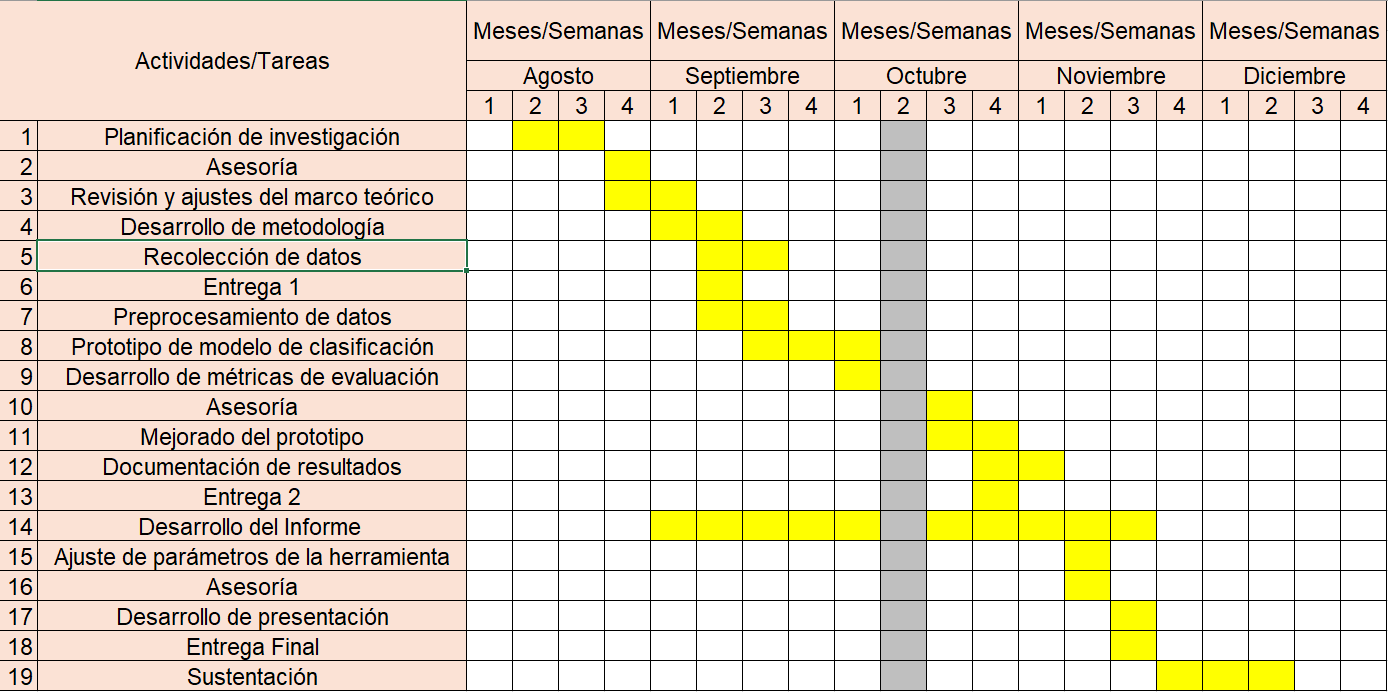
\includegraphics[width=1\textwidth]{3/figures/Gantt.png}
	\caption{Cronograma de actividades del proyecto.}
	\label{fig:cronograma_actividades}
\end{figure}


\section{Presupuesto}
El presupuesto del proyecto, como se detalla en la Tabla \ref{tabla
}, incluye los recursos materiales, técnicos y de servicios necesarios para su ejecución exitosa. Los costos están distribuidos en diferentes categorías: Hardware, que abarca equipos de cómputo esenciales; Software, centrado en herramientas de código abierto como Python; y Servicios, que incluye los gastos de conectividad a internet y suministro eléctrico. Este desglose permite visualizar los recursos disponibles y asegurar que el proyecto disponga de los medios necesarios para cumplir con sus objetivos de manera eficiente.

\begin{table}[H]
	\centering
	\caption{\textit{Presupuesto del Proyecto}}
	\begin{adjustbox}{max width=\textwidth}
	\begin{tabular}{p{2cm}p{3cm}p{3cm}p{4.5cm}p{4cm}p{2cm}}
		\hline
		\textbf{Tipo} & \textbf{Categoría} & \textbf{Recurso} & \textbf{Descripción} & \textbf{\raggedright Fuente Financiadora} & \textbf{Monto (Soles)} \\ \hline
		Hardware & Computadoras & Laptop & Computadora portátil con capacidad de procesamiento avanzado & Propio & 6,000 \\ 
		Software & Procesamiento & Python & Lenguaje de programación de código abierto & - & - \\
		Servicio & Conectividad & Internet & Conexión a internet de alta velocidad para uso de herramientas y recursos online & Propio & 900 \\
		Servicio & Conectividad & Electricidad & Suministro de energía eléctrica para los equipos durante el procesamiento de datos & Propio & 1,200 \\ 
		\textbf{Total} & & & & & \textbf{8,100} \\ 
		\hline
	\end{tabular}
	\end{adjustbox}
	\label{tabla:presupuesto}
\end{table}
